\documentclass[a4paper]{article}
\usepackage{unifrrr}
\usepackage{graphicx}
\usepackage[latin1]{inputenc}
\usepackage{float}
\usepackage[colorlinks=false, pdfborder={0 0 0}]{hyperref}
\usepackage{verbatim}
\usepackage{hyperref}
\usepackage{cite}
\usepackage[english]{babel}
\usepackage{listings}
\usepackage{color}
\definecolor{javared}{rgb}{0.6,0,0} % for strings
\definecolor{javagreen}{rgb}{0.25,0.5,0.35} % comments
\definecolor{javapurple}{rgb}{0.5,0,0.35} % keywords
\definecolor{javadocblue}{rgb}{0.25,0.35,0.75} % javadoc


\lstset{language=Java,
basicstyle=\ttfamily,
keywordstyle=\color{javapurple}\bfseries,
stringstyle=\color{javared},
commentstyle=\color{javagreen},
morecomment=[s][\color{javadocblue}]{/**}{*/},
numbers=left,
numberstyle=\tiny\color{black},
stepnumber=2,
numbersep=10pt,
tabsize=4,
showspaces=false,
showstringspaces=false}

\begingroup
    \catcode `\@ = 11
    \catcode `\~ = 13
    \catcode `\% = 12
    \protected\long\gdef\cmt@remove#1%~{\endgroup}
    \ifdefined~
        \global\let\cmt@old~
    \else
        \global\let\cmt@old\relax
    \fi
    \protected\gdef~{\begingroup\catcode`%=12
        \futurelet\next\cmt@}
    \protected\gdef\cmt@
      {\ifx%\next
           \expandafter\cmt@remove
       \else
           \endgroup\expandafter\cmt@old
       \fi}
\endgroup


\setcounter{secnumdepth}{4}
\setcounter{tocdepth}{4}

%--------------------------------------------------------------------


%The body of the LaTeX file
\begin{document}  



%Including of the title page. See titlepage.tex file
%Autor: Daniel Fasel daniel.fasel@unifr.ch
%Date: 10.01.2008
%Comment: An example of a title page file

%Starting the title page. A \begin command always ends with a \end command
\begin{titlepage} 
	%Center all the following stuff
	\begin{center}
		
		%Include the unifr.jpg file from ./images. \\ is a line break
		
\includegraphics[scale=2]{images/unifr.jpg}\\
		
		%Do a vertical space of 0.5 cm
		\vspace{0.5cm}
		
		
	
		\vspace{2cm}
		
		\begin{Large}
		Seminar Thesis: Applying Fuzzy Logic to Data Warehouses\\
		\end{Large}
		
		\vspace{2cm}
		
		%Start a huge font
		\begin{huge}
			%Sans serif
			{\sf \bf Fuzzy Concepts on Real Time Applications}
		\end{huge}
		
				
		\vspace{2cm}
		
		 %N\"uesch in capitals
		 Steve ASCHWANDEN \\
		 Stefan \textsc{N\"UESCH}\\
		
		\vspace{1.5cm}
		
		{\bf Examiner}\\
		Dr. Daniel Fasel\\
		\vspace{2.5cm}
		
		
		Wabern, \today\\
		
				
	\end{center}
\end{titlepage}


\pagenumbering{arabic}
\pagestyle{plain}
\newpage

\tableofcontents
\newpage

\section{Introduction}

The number of new tweets per second on the social media platform Twitter\footnote{https://www.twitter.com} is huge (over hundred thousand per second). To handle such a big amount of data, a scalable, fault-tolerant real-time framework has to be used. Storm was benchmarked at processing one million 100 byte messages per second per node\footnote{http://storm-project.net}. It allows to classify every new tweet, for example with a fuzzy logic approach. The so called ''Spout'' is responsible for fetching the tweets and the ''Bolts'' can do some transformation on the received data or persist them in some sort of storage. Cassandra\footnote{http://cassandra.apache.org} is an ideal solution for the given scenario, because it is a distributed, elastically scalable, highly available, fault-tolerant and column-oriented database.

\subsection{Problem Statement}

\subsubsection{Research Questions}
\vspace{0.5cm}
\begin{itemize}
\item How can fuzzy classifications be applied to twitter feeds using storm?
\item How can the results of such classifications be stored in a cassandra column store?
\end{itemize}



\subsection{Objectives}

The main objective of this seminar project is to develop a simple prototype, which uses storm to fuzzily classify messages from twitter feeds and store the results in a Cassandra NoSQL database.
The resulting application will use Storm on local system only (not on a cluster). Furthermore, only one fuzzy concept will be implemented in combination with a simple semantic analysis of the twitter feeds. However, the prototype shall be easily extensible with more complex analytics and further fuzzy concepts.


\subsection{Methodology}
This thesis will be conducted by prototyping. 
\subsection{Prototype}
The prototype resulting from this project will be a Java application based on the Storm library and using Cassandra for persistence. For analysing the twitter feeds, SentiWordNet will be used. 

\section{Existing Research}
\subsection{Twitter Trends}
There are several papers about twitter trends available. Some interesting approaches will be discussed in this chapter.\\

A few people from the Northwestern University implemented a topic classification algorithm for twitter trends \cite{leeEtAl2011}. To collect data for their experiments they used the information provided by the "What the trend" website. They downloaded tweets which correspond to over 23'000 trending topics and randomly selected 768 topics to assign them to one of 18 selected topic classes like health, politics, technology or movies. They used supervised learning techniques to classify the trends to a topic class. The provided example (Figure \ref{techClass}) shows the hottest topics in the technology class.
\begin{figure}[h!]
	\centering
	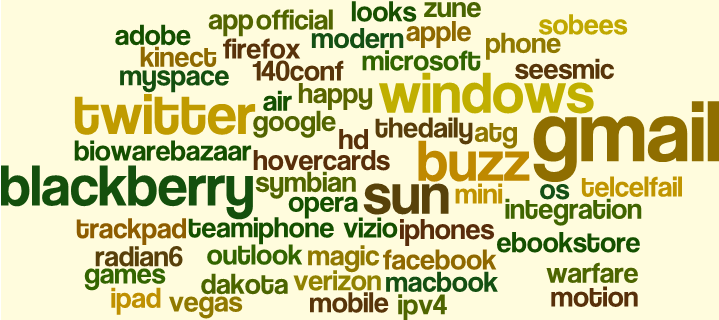
\includegraphics[scale=0.35]{images/technologyClass.png}
	\caption{Technology class topics}
	\label{techClass}
\end{figure}

Another paper has the focus on the trend detection \cite{Mathioudakis2010}. Two guys from the Computer Science department at the University of Toronto developed a monitor (Figure \ref{monitorArchitecture}) for twitter trends in real-time. They split their implementation into a front and back-end part. The TwitterListener separates the tweet information into fields (tweet text, author, timestamp) and exports feeds. Text and timestamp goes to the Bursty Keywords Detection module. This module computes a set of bursty keywords for every tweet and tries to find other tweets in the past which were assigned to the same set (Bursty Keywords Grouping). If the system has found enough tweets it will create a new trend with the corresponding description (Trend Analysis). The Lucene module needs all the fields from the tweet. Apache Lucene is responsible for indexing the tweets. This is important to get feeds from the past, because the Twitter API had some restrictions for requests that date further back in time. The Interface module will present the trends on a webpage.
\begin{figure}[h!]
	\centering
	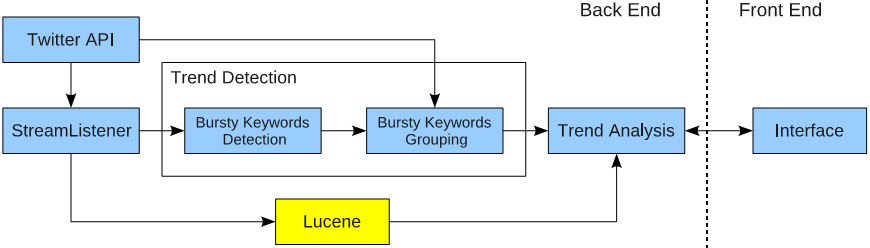
\includegraphics[scale=0.45]{images/monitorArchitecture.png}
	\caption{Architecture of the Twitter Monitor}
	\label{monitorArchitecture}
\end{figure}

\subsection{Sentiment Analysis}
The sentiment analysis of a tweet is also a well-covered topic by the computer science community.\\ 

Members of the University of Edinburgh wrote a paper with the title: "Twitter Sentiment Analysis: The Good, the Bad and the OMG!" \cite{KouloumpisWM11}. They took tweets and did some preprocessing steps first. Replace abbreviations by their actual meaning (e.g. 'BRB' goes to 'be right back') and repeated characters are replaced by single characters (e.g. 'happyyyy' goes to 'happy'). Finally, each word was assigned to a POS-tag (Part-of-Speech). After that, a number of feature values was calculated. The n-gram feature which is a contiguous sequence of n items from a given tweet. The Part-of-Speech feature count the number of verbs, adverbs, adjectives, nouns and any others. The MPQA subjectivity lexicon (similar to SentiWordNet) was used to calculate a positive, negative and neutral value based on the presence of any words from the lexicon. Emoticons and abbreviations - Micro-blogging feature - define a feature too (by the use of the Internet Lingo Dictionary and various internet slang dictionaries). To train an AdaBost model they used over 20'000 tweets. The usage of the Part-of-Speech feature didn't improve the performance of the classifier. The micro-blogging feature was clearly the most useful. With the best combination of the features they get an average accuracy of 0.75 on different test sets (Figure \ref{sentimentAccuracy}).
\begin{figure}[h!]
	\centering
	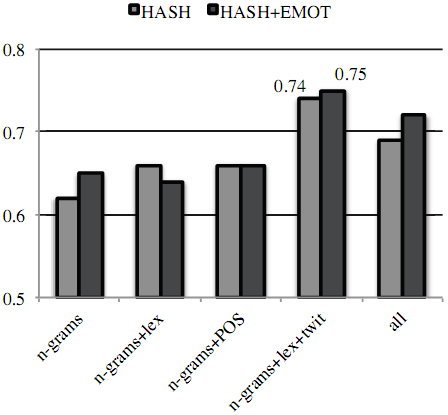
\includegraphics[scale=0.5]{images/sentimentAccuracy.png}
	\caption{Average accuracy with different features}
	\label{sentimentAccuracy}
\end{figure}

\subsection{SentiWordNet}

\section{Technologies}

\subsection{Storm}
Storm is an open source distributed real-time computation system and programming language independent with the following nice properties:
\begin{itemize}
	\item \textbf{Easy to program} An implementation of a real-time processing tool from scratch needs a lot of time and effort. With storm, a simple working topology can be created within a few hours 
	\item \textbf{Programming language independent} The easiest way is to develop in a JVM-based language, but Storm support any language if you use or implement a small intermediate library 
	\item \textbf{Fault-tolerant} If a worker is going down, the cluster will reassign tasks when necessary 
	\item \textbf{Scalable} Add or remove machines to the cluster. Storm will reassign tasks to new machines as the are available or distribute the tasks from the removed machines to the others which are still there 
	\item \textbf{Reliable} Storm guarantees that every message will processed at least once. If an error occurs, the messages can be processed more then once. But a message will never be lost 
	\item \textbf{Fast} Storm can process one million 100 byte per second per node on a machine with two processors (Intel E5645@2.4Ghz) and a 24 GB memory 
\end{itemize}
\subsubsection{Components}
A storm topology consists of two main components:
\begin{itemize}
	\item Spouts are responsible to fetch the data from a source (e.g. text file, twitter streaming API)
	\item Bolts are responsible for the transformations of the fetched data
\end{itemize}
The spout acts as the source of the data flow and the last bolt is the sink which store the output to a database. The output of one component goes always to the input of the next, therefore no data will flow through an already visited node. A simple example should help to illustrate the components of the storm architecture (Figure \ref{storm_example}):\\

\begin{figure}[h!]
	\centering
	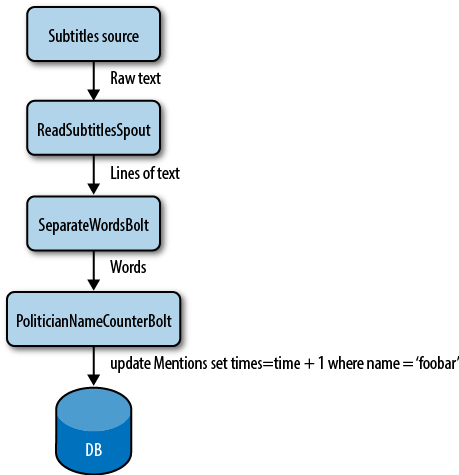
\includegraphics[scale=0.5]{images/storm_example.png}
	\caption{Storm example}
	\label{storm_example}
\end{figure}
All the spoken words during the TV news show will be stored in a text file. If a new sentence was written into the file the spout hands them to the responsible bolt which separate the sentence into words. This stream of words is passed to another bolt that compares each word to a list of politician's names. If there is a match, the second bolt increases the counter for that name in a storage. To check the number of occurrence, query the database which is updated in real-time.\\
Typical uses cases for a storm application can be:
\begin{itemize}
	\item \textbf{Processing streams} This is the case in shown example 
	\item \textbf{Continuous computation} Send continuously data to the clients so they can update and display results in real-time, for example as site metrics 
	\item \textbf{Distributed remote procedure call} Easily parallelize CPU-intensive operations
\end{itemize}
\subsubsection{Grouping}
After the implementation of the spouts and bolts for the topology, they have to be connected with each other. Stream grouping defines which stream are consumed by each bolt and how they will be consumed. Strom provides different grouping types: 
\begin{itemize}
	\item \textbf{Shuffle} The most commonly used grouping. It sends each tuple emitted by the source to a randomly chosen bolt. If there are no dependencies between the emitted tuples (e.g. fuzzy classification of a tweet) this grouping method is used 
	\item \textbf{Fields} Control how the tuples will be distributed, based on the emitted fields. It guarantees that a set of values for the same combination of fields will be sent to the same bolt. This is useful to implement a MapReduce functionality 
	\item \textbf{All} Sends a single copy of each tuple to every receiving bolt (e.g. resetting a counter, refreshing a cache) 
	\item \textbf{Custom} Create a custom stream grouping by implementing the\\
\textit{back.type.storm.grouping.CustomStreamGrouping} interface 
\end{itemize}
\subsubsection{Technical Details}
In a storm cluster there are 2 node types, a master node and worker nodes. On the master node runs a daemon called 'Nimbus', which is responsible for code distribution, assigning tasks to the worker nodes and failure monitoring. A portion of the topology is running on the worker nodes (responsible daemon is called 'Supervisor'). A topology runs across multiple worker nodes on different machines. Since Storm keeps the states of the cluster either in 'Zookeeper' or on local disk, the daemons are stateless and can fail or restart without disturbing the system.\\
Storm uses an advanced, embeddable networking library zeromq (0mq, http://zeromq.org/), which provides features that make Storm possible. Some characteristics of zeromq:
\begin{itemize}
	\item Act as a concurrency framework
	\item Faster than TCP, ideal for clustered products and supercomputers
	\item Carries messages across in-process, IPC (inter-process communication), TCP and multicast
	\item Asynchronous I/O model for scalable multi-core applications
	\item Connect sockets N-to-N 
\end{itemize}
Storm topologies can run in two different modes. The local mode is a single Java Virtual Machine on a local machine. This mode is used for developing, testing and debugging. The other possibility is to run the software on different remote machines. But there are no debugging information in the production mode.\\

The difference between a traditional BigData approach like Hadoop and storm is the paradigm that it addresses. Hadoop fundamentally a batch processing system. The results are available after the whole data was distributed over the whole system. The construction of topologies that transform unterminated streams of data is supported by storm. A storm topology will never stop running (until termination by user), Hadoop jobs will stop after all available data (at starting time) proceeded by the system.

\subsection{Cassandra}
Eben Hewitt explained Cassandra with only 50 words \cite{hewitt2010cassandra}:\\

"Apache Cassandra is an open source, distributed, decentralized, elastically scalable, highly  available, fault-tolerant, tuneably consistent, column-oriented database that bases its distribution design on Amazon's Dynamo and its data model on Google's Bigtable. Created at Facebook, it is now used at some of the most popular sites on the Web."\\

The data store is an open source Apache project available at http://cassandra.apache.org. Cassandra originated at Facebook in 2007. It should solve the company's inbox search problem, because they had to deal with large volumes of data. The project was moved to Apache in March 2009. Cassandra has some interesting properties:

\subsubsection{Elastic Scalability }
There are two different types of scaling. Add more hardware capacity and memory to the existing way is one way to handle a greater number of requests. This approach is called vertical scaling. Horizontal scaling will add more machines to distributed the incoming data over multiple nodes. This will decrease the amount of data for every machine. Elastic scalability is a specialization of the horizontal scaling where the cluster can scale up and scale back down, depending on the current load. Cassandra is able to handle new machines on-the-fly, no restart of the process or manually rebalancing of the data is required. 
\subsubsection{High Availability and Fault Tolerance}
Machines in the cluster will have technical issues from time to time. Cassandra is able to handle replaced failed nodes without downtime. Also replication of data to multiple data center is possible to prevent downtime if a data center experiences a catastrophe like a fire. 
\subsubsection{Tuneable Consistency}
Consistency means that a read operation returns the last written value from the database. But a database system cannot implement all three components of the CAP theorem and the focus of Cassandra are Availability and Partition tolerance (AP). Therefore, the consistency is not guaranteed. But it allows to configure the degree of the consistency in balance with the level of availability: 
\begin{itemize}
	\item \textbf{Strict consistency} Also called sequential consistency. It's the highest level of consistency and it requires that a read will always return the recently written value in the database. If you have only a single machine with one processor (and one processor clock) the last written value is easy to find. But if there are geographically dispersed data centers, it becomes much more slippery. A global clock which can timestamp all operations, regardless of the data location or how many services are needed to determine the response, is required 
	\item \textbf{Causal consistency} A weaker form of the strict approach. It uses a much more semantic approach and it does away with the fantasy of a single clock which can be synchronized without creating a bottleneck. The idea is that writes which are potentially related must be read in sequence. Writes are inferred not to be causally related, if two operations suddenly write to the same filed (operations must be different and unrelated). But if there is enough time between two write operations, we assume that they are causally related. Therefore, causal consistency says that causal writes must be read in sequence 
	\item \textbf{Weak (eventual) consistency} All updates will propagate throughout all of the machines in a distributed system. Of course, this will take some time. But It could be possible that all replicas will be consistent 
\end{itemize}
The user of Cassandra can control the number of replicas to block on for all updates (Tunable consistency). This can be done by setting the level of consistency against the replication factor. With the replication factor the client can define the level of consistency, but a higher level implies a lower performance of the system. The factor controls the number of nodes in the cluster where you want to distribute the updates (add, update and delete). The number of replicas which have to acknowledge a write operation or respond to a read operation to declare this operation as successful is defined by the consistency level.

\subsubsection{Raw-Oriented}
Cassandra is a column-oriented database, it represents it's data structures in sparse multidimensional hashtables. For every given row you can have many columns, but they doesn't have to be the all the same like in the relational model. A unique key makes the data accessible. One advantage of Cassandra is that you don't have to define what the data structure must look like or what fields you will need. This implies also that you can add or remove new fields on the fly without disturbing the system. This is ideal if you use an agile development methodology and you don't have time to define the entire database schema at the beginning of the project.

\subsubsection{Schema-Free}
The first step to define a Cassandra database is the creation of a keyspace which is a logical namespace to hold column families and some configuration properties.

\subsubsection{High Performance}
Cassandra was designed to take full advantage of multiprocessor/multicore machines and run on multiple of these machines in data centers. It should be scale to hundreds of terabytes and stay consistent. People from the university of Toronto analysed the performance of Cassandra \cite{rabEtAl2012}. They defined some different workloads to create some scenarios. One was with 50\% inserts, 25\% reads and 25\% scans. Two independent clusters are used where each has about 16 Linux nodes (Intel Xeon quad core CPU's, 16GB of RAM, 148GB disk space). The nodes are connected with a gigabit Ethernet network over a single switch. The strength of Cassandra is clearly visible (Figure \ref{throughput_cassandra}), because the throughput with only one node is lower than other ones. If the number of nodes was increased, the gap between Cassandra and all the other tested systems is huge.

\begin{figure}[h!]
	\centering
	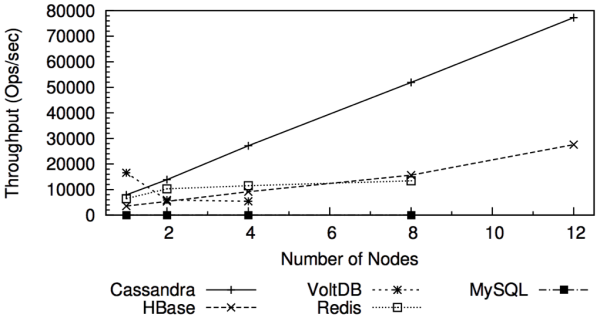
\includegraphics[scale=0.5]{images/throughputCassandra.png}
	\caption{Performance of different distributed database systems}
	\label{throughput_cassandra}
\end{figure}

The authors of the paper concluded their paper with the following words:\\

"In terms of scalability, there is a clear winner throughout our experiments. Cassandra achieves the highest throughput for the maximum number of nodes in all experiments with a linear increasing throughput from 1 to 12 nodes."

\section{Implementation}
\subsection{Architecture}
\subsection{SentiWordNet Analysis}
SentiNetWord is an English dictionary for opinion mining (OM, also known as sentiment classification). The goal was to decide for every word of the WordNet if it has a positive, negative or neutral meaning. WordNet is a large lexical database of nouns, verbs, adjectives and adverbs provided by the Princeton University. The developers calculated for every word three values between 0.0 and 1.0 and they had to sum up to one. They labelled different entries of the dictionary manually to define a ground truth for the training set. Then a set of classifiers was trained with the provided data. After these steps the classifiers were able to calculate the corresponding values of the remaining words which weren't in the training data samples. Since the first version of SentiWordNet in 2006 a lot of improvements are done, the actual version is 3.0.0. It's freely available for research approaches.\\
The dictionary consists of 117'659 entries (69.8\% nouns, 15.4\% adjectives, 11.7\% verbs and 3.1\% adverbs). If we take a closer look at the calculated values (in SentiNetWord 1.0.0) we can see that most of the words are objective (about eighty percent are greater than 0.75). Only a few words are positive (0.48\% \textgreater \ 0.75; about 560 words) or negative (1.28\% \textgreater \ 0.75; about 1500 words).\\
The resulting dictionary can be downloaded on the research website of SentiWordNet and has the following columns (tab separated):
\begin{enumerate}
	\item Part of speech (noun, verb, adjective, adverb)
  \item ID
	\item Positive score
	\item Negative score
	\item The words (plural because of synonyms)
	\item Glossary (the word in a given context)
\end{enumerate}
The neutral (objective) score of the word can be calculated by 1 - (Positive score + Negative score).

\subsection{Fuzzy Concept Implementation}
To delegate the creation of the model with the implemented fuzzy approach to the \textit{FuzzyBolt} class, a Parameterized Factory Method pattern is used. It's possible to create a new fuzzy model approach by extending the \textit{FuzzyModel} class and modify the \textit{FuzzyModelFactory} to make the object creation of the corresponding model accessible. The selection of the new approach can be done by the following statements:
\lstset{language=Java}
\begin{lstlisting}
FuzzyBolt fuzzyBolt = new FuzzyBolt();
fuzzyBolt.setFuzzyModelName(``our approach'');
\end{lstlisting}
The second line will call the static \textit{getFuzzyModel} method of the factory.
The \textit{SentiWordFuzzyModel} class has a \textit{createDict} method which creates a hash map out of the text file consists of the word as key and the corresponding vector with the opinions (positive, negative and neutral) as value.
The \textit{FuzzyBolt} class is the first bolt in the whole Storm process and receives the output of the twitter spout. The execute-method calculates the three sentiment values of the tweet and give them to the Cassandra bolt.

\subsection{Topology}
\begin{figure}[h!]
	\centering
	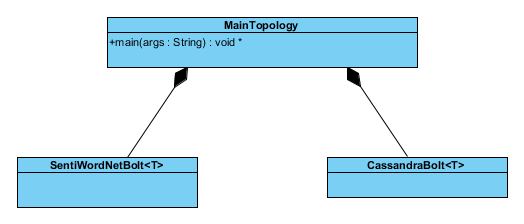
\includegraphics[scale=2.5]{images/uml_topology.png}
	\caption{Class Diagram of the implemented topology}
	\label{uml_fuzzy}
\end{figure}
\subsection{Data Collection}
\subsection{Classification}
\subsubsection{Discrete Classification}
\begin{figure}[h!]
	\centering
	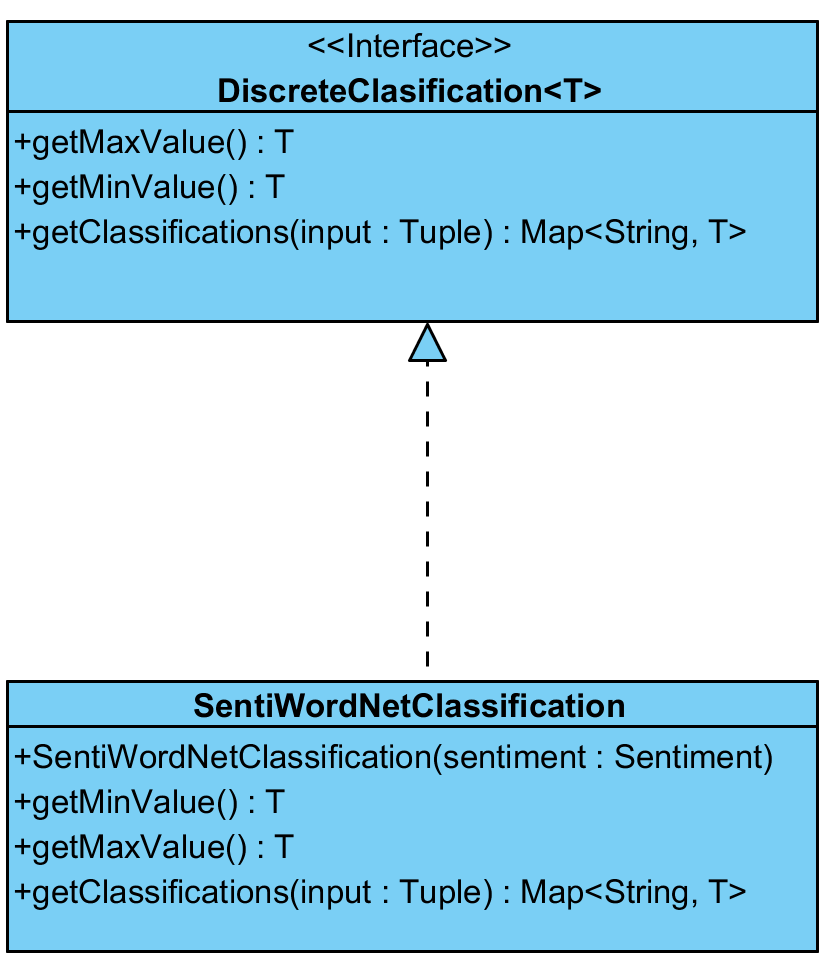
\includegraphics[scale=2.5]{images/uml_discrete.png}
	\caption{Discrete Classification - Interface and Sample Implementation}
	\label{uml_fuzzy}
\end{figure}
\subsubsection{Fuzzy Classification}
\begin{figure}[h!]
	\centering
	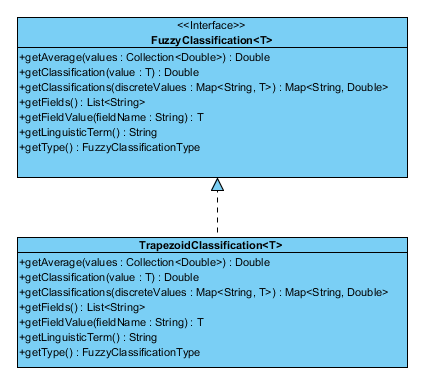
\includegraphics[scale=2.5]{images/uml_fuzzy.png}
	\caption{Fuzzy Classification - Interface and Sample Implementation}
	\label{uml_fuzzy}
\end{figure}
\begin{figure}[h!]
	\centering
	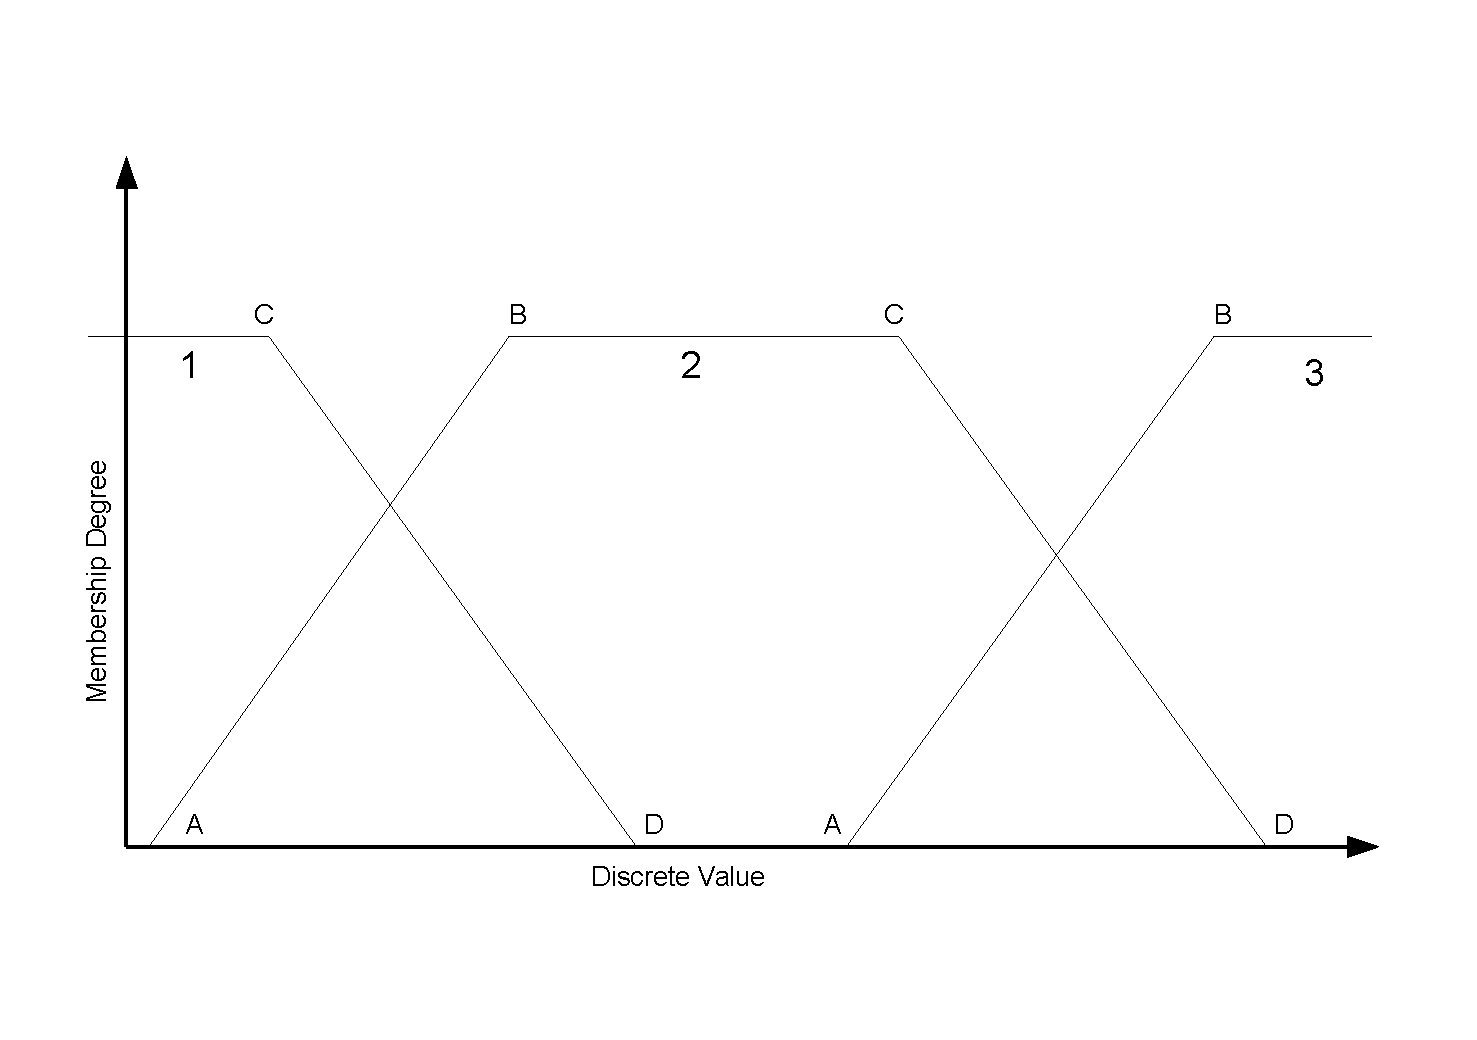
\includegraphics[scale=0.5]{images/trapezoid.pdf}
	\caption{Trapezoid Member ship function (based on \cite{faseld2012}, p. 74)}
	\label{trapezoid_functions}
\end{figure}
\subsection{Persistence}
\subsection{Build Infrastructure}
\subsection{Extensibility: API}

\section{Conclusion}



\newpage



\section{References}
\selectlanguage{English}
\bibliographystyle{plain}
\bibliography{references}

\newpage
~%
\bibliography{diva_group}
\bibliographystyle{plain}

\addcontentsline{Tc}{section}{Bibliography}

\begin{thebibliography}{20}

	\bibitem{senti}
	Andrea Esuli, Fabrizio Sebastiani
	\newblock{\em SentiWordNet: A Publicly Available Lexical Resource for Opinion Mining}
	\newblock available: \url{http://sentiwordnet.isti.cnr.it/}, accessed 18th November 2013.
	
	\bibitem{senti3}
	Stefano Baccianella, Andrea Esuli, Fabrizio Sebastiani
	\newblock{\em SentiWordNet 3.0: An Enhanced Lexical Resource for Sentiment Analysis and Opinion Mining}
	\newblock available: \url{http://sentiwordnet.isti.cnr.it/}, accessed 18th November 2013.
	
	\bibitem{twitter}
	Alec Go, Lei Huang, Richa Bhayani
	\newblock{\em Twitter Sentiment Analysis}
	\newblock available: \url{http://www-nlp.stanford.edu/courses/cs224n/2009/fp/3.pdf}, accessed 18th November 2013.
	
	\bibitem{twitterStorm}
	M. Tim Jones
	\newblock{\em Process real-time big data with Twitter Storm}
	\newblock available: \url{http://www.ibm.com/developerworks/library/os-twitterstorm/os-twitterstorm-pdf.pdf}, accessed 18th November 2013.
	
	\bibitem{stormCassandra}
	Shalom N. 
	\newblock{\em Nati Shalom's Blog: Real-Time Big Data with Storm, Cassandra, and XAP; April 4th, 2013}
	\newblock available: \url{http://natishalom.typepad.com/nati_shaloms_blog/2013/04/real-time-big-data-with-storm-cassandra-and-xap-1.html}, accessed 18th November 2013.

	\bibitem{stormBook}
	Jonathan Leibiusky, Gabriel Eisbruch and Dario Simonassi 
	\newblock{\em Getting Started with Storm;}
	\newblock 30th August 2012; O'Reilly, 978-1-449-32401-8

	\bibitem{cassandraBook}
	Eben Hewitt 
	\newblock{\em Cassandra - The Definitive Guide;}
	\newblock November 2010; O'Reilly, 978-1-449-39041-9

	\bibitem{perfCassandra}
	Tilmann Rabl, Mohammad Sadoghi, Hans-Arno Jacobsen, Sergio Gomez-Villamor, Victor Muntes-Mulero, Serge Mankovskii
	\newblock{\em Solving Big Data Challenges for Enterprise Application Performance Management}
	\newblock available: \url{http://vldb.org/pvldb/vol5/p1724_tilmannrabl_vldb2012.pdf}, accessed 2nd December 2013.

	\bibitem{classTwitterTrends}
	Kathy Lee, Diana Palsetia, Ramanathan Narayanan, Mostofa Ali Patwary, Ankit Agrawal, and Alok Choudhary
	\newblock{\em Twitter Trending Topic Classification}
	\newblock available: \url{http://cucis.eecs.northwestern.edu/publications/pdf/LeePal11.pdf}, accessed 3nd December 2013.

	\bibitem{monitorTwitterTrends}
	Michael Mathioudakis, Nick Koudas
	\newblock{\em TwitterMonitor: Trend Detection over the Twitter Stream}
	\newblock available: \url{http://snap.stanford.edu/class/cs224w-readings/mathioudakis10twitter.pdf}, accessed 3nd December 2013.
	
	\bibitem{sentimentAnalysisEdin}
	Efthymios Kouloumpis, Theresa Wilson, Johanna Moore
	\newblock{\em Twitter Sentiment Analysis: The Good the bad and the OMG!}
	\newblock available: \url{http://crowdsourcing-class.org/assignments/downloads/kouloumpis-et-al.pdf}, accessed 3nd December 2013.
	
	\bibitem{faseld2012}
	Daniel Fasel
	\newblock{\em Concept and Implementation of a Fuzzy Data Warehouse}
	\newblock Doctoral Thesis, Switzerland, May 2012.

	\newblock{}
	\newblock{}
	
\end{thebibliography}
%~



\end{document}
